\documentclass[a4paper,11pt]{article}

%%%%%%%%%%%%%%%%%%%%%%%%%%%%%%%%%%%%%%%%%%%%%%%%%%%%%%%%%%%%%%%%%%%%%%%%
% Paquetes utilizados
%%%%%%%%%%%%%%%%%%%%%%%%%%%%%%%%%%%%%%%%%%%%%%%%%%%%%%%%%%%%%%%%%%%%%%%%

\usepackage[margin=0.8in]{geometry}

% Gráficos complejos
\usepackage{graphicx}
\usepackage{caption}
\usepackage{subcaption}
\usepackage{placeins}

% Soporte para el lenguaje español
\usepackage{textcomp}
\usepackage[utf8]{inputenc}
\usepackage[T1]{fontenc}
\DeclareUnicodeCharacter{B0}{\textdegree}
\usepackage[spanish]{babel}

% Código fuente embebido
\usepackage{listings}
\usepackage{courier}

% PDFs embebidos para el apéndice
\usepackage{pdfpages}

% Matemáticos
\usepackage{amssymb,amsmath}

% Tablas complejas
\usepackage{multirow}

% Formato de párrafo
\setlength{\parskip}{1ex plus 0.5ex minus 0.2ex}

% Subrayado de palabras
\usepackage[normalem]{ulem}

% Agregados en el documento
\usepackage{array}
\usepackage{fancyhdr}
\renewcommand{\headrulewidth}{0pt}
\renewcommand{\footrulewidth}{0pt}

% Formato de listados de código
\lstset{
  basicstyle=\footnotesize\ttfamily,
  numberstyle=\tiny,
  numbersep=5pt,
  tabsize=2,
  extendedchars=true,
  breaklines=true,
  stringstyle=\color{white}\ttfamily,
  showspaces=false,
  showtabs=false,
  xleftmargin=17pt,
  framexleftmargin=17pt,
  framexrightmargin=5pt,
  framexbottommargin=4pt,
  showstringspaces=false,
  language=SQL
}
\usepackage{caption}
\DeclareCaptionFont{white}{\color{white}}
\DeclareCaptionFormat{listing}{\colorbox[cmyk]{0.43, 0.35, 0.35,0.01}{\parbox{\textwidth}{\hspace{15pt}#1#2#3}}}
\captionsetup[lstlisting]{format=listing,labelfont=white,textfont=white, singlelinecheck=false, margin=0pt, font={bf,footnotesize}}

%%%%%%%%%%%%%%%%%%%%%%%%%%%%%%%%%%%%%%%%%%%%%%%%%%%%%%%%%%%%%%%%%%%%%%%%
% Título
%%%%%%%%%%%%%%%%%%%%%%%%%%%%%%%%%%%%%%%%%%%%%%%%%%%%%%%%%%%%%%%%%%%%%%%%
% Título principal del documento.

\title{\textbf{Trabajo Práctico: Agenda Médica}}

% Información sobre los autores.
\author{
  Celeste Maldonado,	\textit{P. 85.630},	\textit{maldonado.celeste@gmail.com}	\\
  Gisela Daye,		\textit{P. 87.602},	\textit{gisedaye@gmail.com}		\\
  Sergio Matías Piano,	\textit{P. 85.191},	\textit{smpiano@gmail.com}		\\
  Vanesa Conte,		\textit{P. 82.997},	\textit{vanexius@gmail.com}		\\
  \\
  \normalsize{Grupo 19}							\\
  \normalsize{Docente: Luis Fulco}					\\
  \normalsize{1er. Cuatrimestre de 2014}                           	\\
  \normalsize{75.15 - Bases de datos}                              	\\
  \normalsize{Facultad de Ingeniería, Universidad de Buenos Aires}
}
\date{}
%%%%%%%%%%%%%%%%%%%%%%%%%%%%%%%%%%%%%%%%%%%%%%%%%%%%%%%%%%%%%%%%%%%%%%%%
% Documento
%%%%%%%%%%%%%%%%%%%%%%%%%%%%%%%%%%%%%%%%%%%%%%%%%%%%%%%%%%%%%%%%%%%%%%%%

\begin{document}

% ----------------------------------------------------------------------
% Top matter
% ----------------------------------------------------------------------
\thispagestyle{empty}

\null  % Empty line
\nointerlineskip  % No skip for prev line
\vfill
\let\snewpage \newpage
\let\newpage \relax

\maketitle

\begin{abstract}

  Este informe resume el desarrollo del trabajo práctico de la materia Base
  de Datos (75.15) dictada en el primer cuatrimestre de 2014 en la Facultad de
  Ingeniería de la Universidad de Buenos Aires. El mismo consiste en el
  modelado de datos de un software de agenda médica,
  cuyos requisitos fueron extraído de un caso de estudio real.

\end{abstract}

\let \newpage \snewpage
\vfill 
\break % page break
\clearpage

% ----------------------------------------------------------------------
% Tabla de contenidos
% ----------------------------------------------------------------------
\tableofcontents
\clearpage


% ----------------------------------------------------------------------
% Desarrollo
% ----------------------------------------------------------------------
\part{Desarrollo}


\section{Modelo de entidad-interrelación} \label{sec:der}

\subsection{Hipótesis}

\begin{enumerate}

    \item Se entiende por demanda espontanea, que el paciente se presenta 
    fisicamente y pide el turno el mismo día.
    
    \item Los turnos los solicita el paciente y los recursos son autorizados 
    solamente por los profesionales.
    
    \item Los hospitales o clínicas aceptan todas las obras sociales.
    
    \item La duración del procedimiento médico se diferencia por especialidad
    y no por subespecialidad del profesional.
    
    \item Se reserva al menos 2 consultas por día para demanda espontanea.
    Éstos 2 turnos se van a encontrar al finalizar la agenda. La idea corresponde
    a que el hospital o clínica esté con la posibilidad de antender la demanda
    espontanea.
    
    \item Siempre que se da de alta una especialidad clasifica en una subespecialidad.
    
    \item Suponemos que los bloques hora deben saber si el profesional acepta 
    sobreturnos para poder darle la flexibilidad al profesional por día y semana 
    que decida que días acepta hacer sobreturnos.
    
    \item Cuando un profesional bloquea un bloque de horas, los turnos creadas 
    para dicho bloque, deben ser modificadas. En tal caso, la recepcionista llama
    a cada paciente para reasignar el turno. No se altera el atributo de anulado 
    sobre el turno.
    
    \item Los turnos solamente se asignan por teléfono o personalmente.
    
    \item Los turnos se asignan solamente por Mesa de Turno.
    
    \item Tipo de turno se considera a primera vez, visita subsiguiente, demanda 
    espontánea, cualquier otro 
    tipo que determine profesional, especialidad o servicio.
    
    \item Los turnos se asignan por profesional, procedimiento médico, especialidad
    o servicio o cualquiera de sus combinaciones.
    
    \item Los servicios, quirófanos y camas son solicitados por médicos. No existe 
    el sobreturno en éste caso.
    
    \item Puede existir un mismo domicilio asociado a varios pacientes (ej. familia)
    o profesionales.
    
    \item Los turnos se generarán a partir de los block horas que no se encuentren 
    bloqueados al momento de crear la agenda.
    
    \item Cada profesional está asociado a por lo menos una subespecialidad. No existen 
    profesionales que no esten asociados a alguna subespecialidad.
    
    \item Por cada block de hora existe una sóla forma de atención a pacientes y un 
    sólo tipo de turno.

\end{enumerate}



\subsection{Diagrama de entidad-interrelación}

 En la figura \ref{fig:der} se incluye el diagrama de entidad-interrelación
 final desarrollado para representar el dominio modelado cuyo relevamiento se
 detalla en el enunciado.

\begin{figure}[h!t]
  \centering
  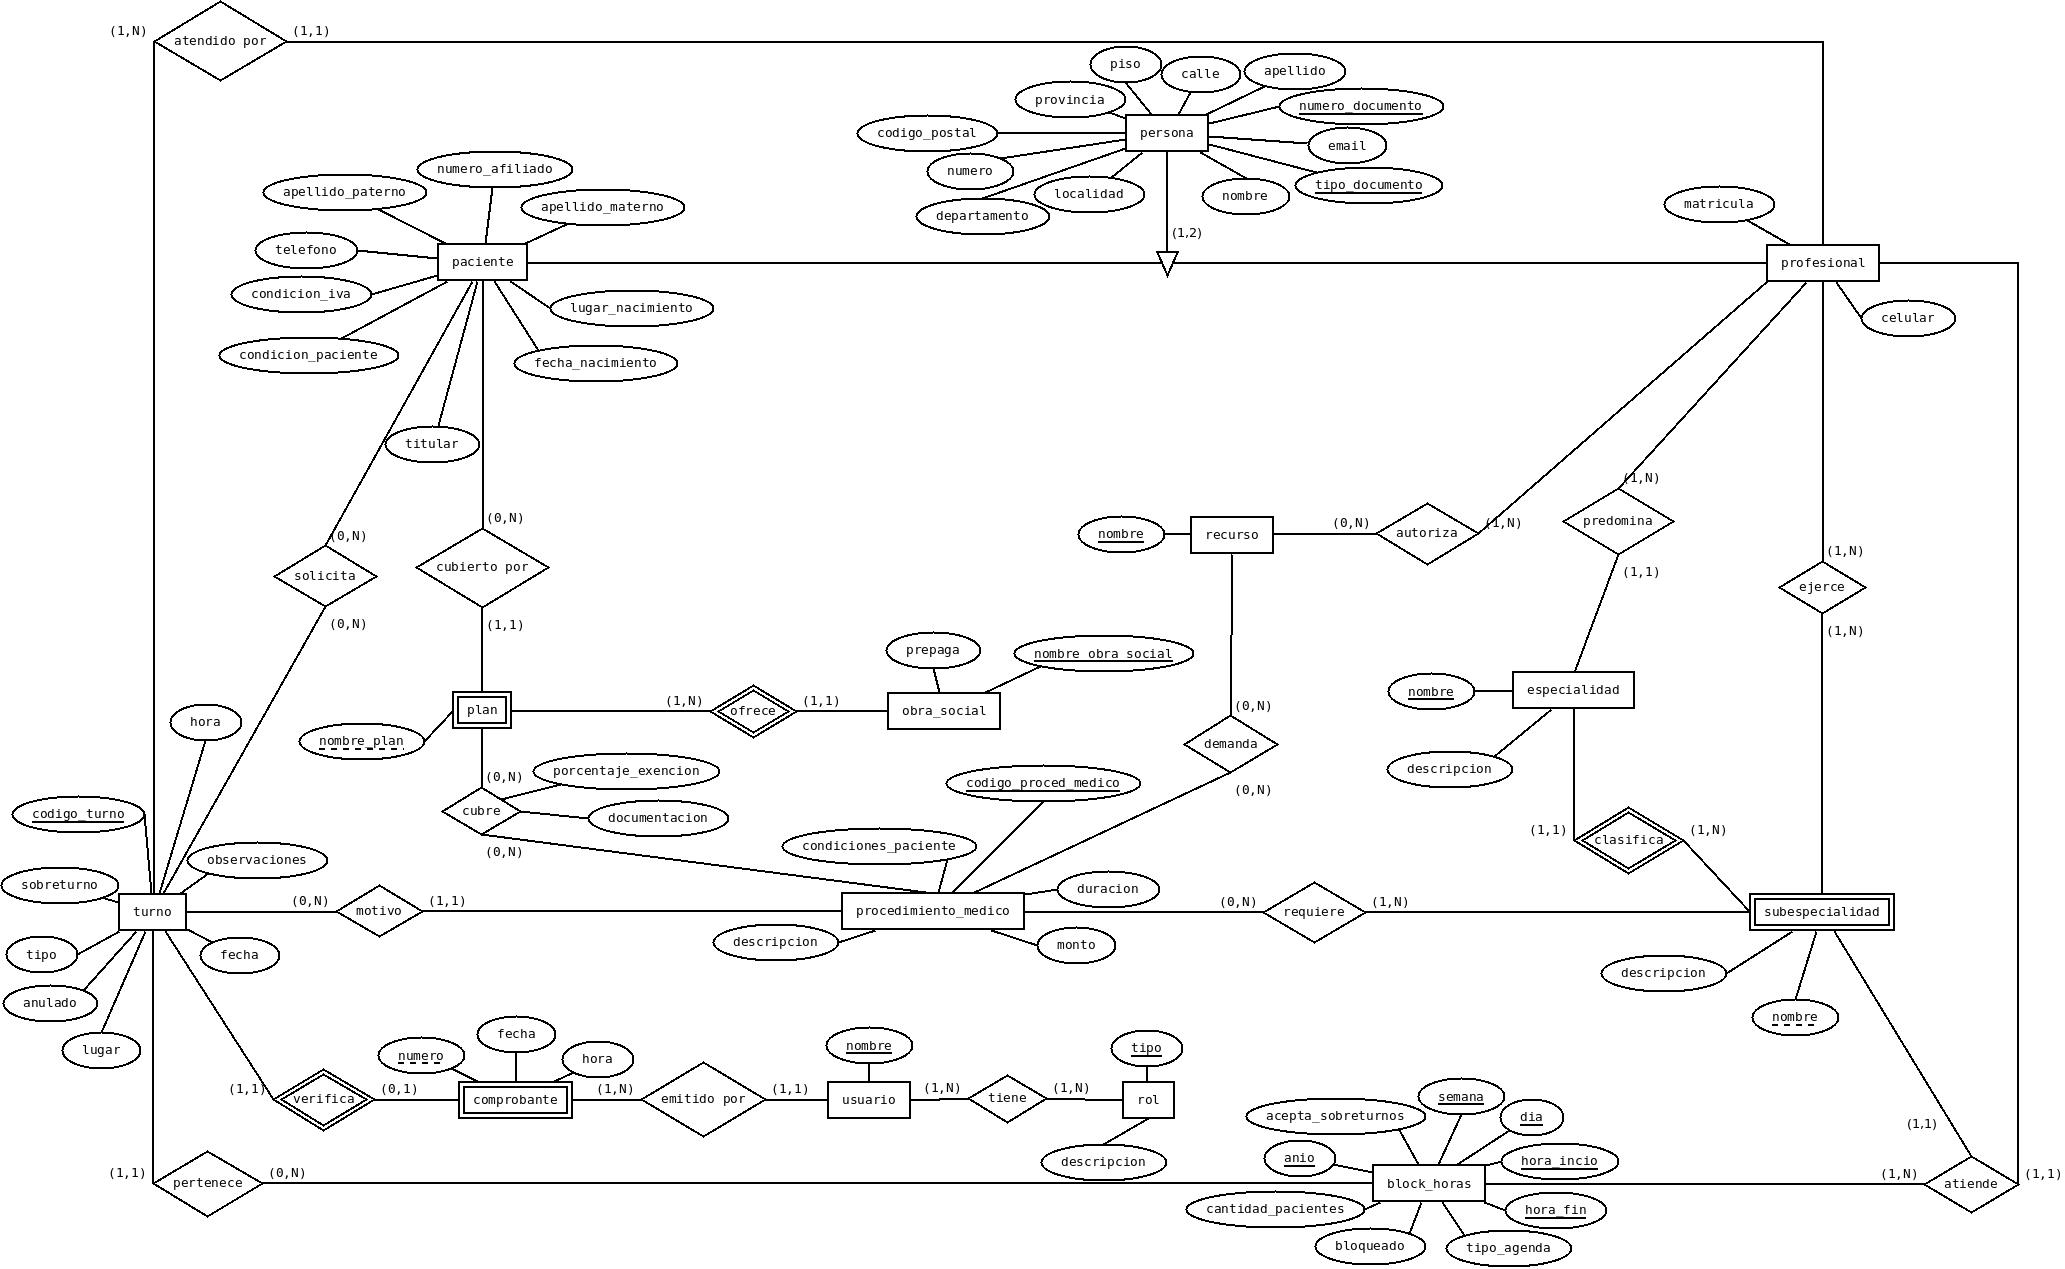
\includegraphics[width=1.4\textwidth, angle=90]{build/images/der.jpeg}
  \caption{Diagrama de entidad-interrelación} \label{fig:der}
\end{figure}

\FloatBarrier


%\section{\textbf{Dependencias}}
%\begin{enumerate}
%\item Existe una dependencia de existencia de la entidad Turno con la entidad Block 
%hora.
%
%\item Existe una dependencia de identidad entre las entidades Plan y Obra social. 
%Plan es una identidad débil, para poder identificarla utilizamos la razón social 
%de la Obra Social (que es clave de la entidad fuerte) y como atributo discriminante 
%el nombre del plan.
%
%\item Existe una dependencia de identidad entre las entidades Especialidad y Subespecialidad. 
%Subespecialidad es una identidad débil, para poder identificarla utilizamos el 
%código de la Especialidad (que es clave de la entidad fuerte) y como atributo 
%discriminante la descripción de la Subespecialidad.
%
%\item Existe una dependencia de identidad entre las entidades Turno y Comprobante. 
%Comprobante es una identidad débil, para poder identificarla utilizamos el código 
%del Turno (que es clave de la entidad fuerte) y como atributo discriminante el 
%número de Comprobante.\pagebreak{}
%\end{enumerate}


\section{\textbf{Diccionario de datos}}

\subsection{\textbf{Entidades}}

\subsubsection{\textbf{paciente}}

\textbf{Definición}

Persona que recibe atención médica en el hospital. Es quién solicita el turno. 

\textbf{Especificación de atributos}

\begin{itemize}

   \item \textbf{numero\_documento:} número de documento del paciente.

   \item \textbf{tipo\_documento:} tipo de documento presentado por el paciente. Puede ser 
   LE, LC, DNI, PASAPORTE.

   \item \textbf{nombre:} nombre del paciente.

   \item \textbf{apellido\_paterno:} apellido paterno del paciente.

   \item \textbf{apellido\_materno:} apellido materno del paciente.

   \item \textbf{fecha\_nacimiento:} día, mes y año en que nació el afiliado.

   \item \textbf{lugar\_nacimiento:} ciudad o pueblo y país donde nació el paciente.

   \item \textbf{telefono:} número de teléfono del paciente.

   \item \textbf{email:} dirección de correo electrónico del paciente.

   \item \textbf{condicion\_iva:} condición del paciente frente al impuesto al valor agregado 
   definido por la AFIP.

   \item \textbf{condicion\_paciente:} estado del paciente.

   \item \textbf{numero\_historia\_clinica:} referencia el número de historia clínica que 
   contiene tratamientos y diagnósticos del paciente.

   \item \textbf{numero\_afiliado:} número asignado al paciente dentro de la obra social.

   \item \textbf{titular:} indica la condición del paciente frente a la obra social. En caso que sea verdadero 
   es titular, sino adicional.
\end{itemize}

\textbf{Especificación de identificador único}

\begin{itemize}

    \item \textbf{tipo\_documento}

    \item \textbf{numero\_documento}

\end{itemize}

\subsubsection{\textbf{domicilio}}

\textbf{Definición}

Lugar donde un PACIENTE o un PROFESIONAL tiene residencia.

\textbf{Especificación de atributos}

\begin{itemize}

     \item \textbf{codigo\_postal:} número que identifica el código postal dónde se ubica el domicilio.

     \item \textbf{provincia:} subdivisión administrativa de un país.

     \item \textbf{localidad:} lugar perteneciente a una PROVINCIA.

     \item \textbf{calle:} nombre de la calle correspondiente al domicilio.

     \item \textbf{numero:} número que identifica al terreno correspondiente al domicilio.

     \item \textbf{piso:} nivel correspondiente al domicilio, en caso de que se trate de un edificio.
\end{itemize}

\textbf{Especificación de identificador único}

\begin{itemize}

     \item \textbf{codigo\_postal}

     \item \textbf{provincia}

     \item \textbf{localidad}

     \item \textbf{calle}

     \item \textbf{numero}

     \item \textbf{piso}

     \item \textbf{departamento}

\end{itemize}

\subsubsection{\textbf{profesional}}

\textbf{Definición}

Un médico del hospital que diagnostica, atiende o trata a un PACIENTE.

\textbf{Especificación de atributos}

\begin{itemize}

     \item \textbf{nombre:} nombre del profesional.

     \item \textbf{apellido:} apellido del profesional.

     \item \textbf{numero\_documento:} número de documento del profesional.

     \item \textbf{tipo\_documento:} tipo de documento presentado por el profesional. Puede ser 
     LE, LC, DNI, PASAPORTE.

     \item \textbf{celular:} número de celular del profesional.

     \item \textbf{email:} dirección de correo electrónico del profesional.

\end{itemize}

\textbf{Especificación de identificador único}

\begin{itemize}

     \item \textbf{tipo\_documento}

     \item \textbf{numero\_documento}

\end{itemize}

\subsubsection{\textbf{especialidad}}

\textbf{Definición}

�rea de la medicina en que se especializa un PROFESIONAL.

\textbf{Especificación de atributos}

\begin{itemize}

     \item \textbf{nombre\_especialidad:} nombre que identifica la especialidad.

     \item \textbf{descripcion:} nombre de la especialidad.

\end{itemize}

\textbf{Especificación de identificador único}

\begin{itemize}

     \item \textbf{nombre}

\end{itemize}

\subsubsection{\textbf{subespecialidad}}

\textbf{Definición}

�rea dentro de la especialidad en que se especializa un PROFESIONAL. Depende de 
la especialidad.

\textbf{Especificación de atributos}

\begin{itemize}

     \item \textbf{nombre\_subespecialidad:} nombre de la subespecialidad.

     \item \textbf{descripcion:} descripción de la subespecialidad.

\end{itemize}

\textbf{Especificación de identificador único}

\begin{itemize}

     \item \textbf{nombre\_especialidad} (especialidad)

     \item \textbf{nombre\_subespecialidad}

\end{itemize}

\subsubsection{\textbf{procedimiento\_medico}}

\textbf{Definición}

Todo procedimiento médico, servicio, estudio o tratamiento brindado por el hospital. 
Incluye servicio de quirófano y camas.

\textbf{Especificación de atributos}

\begin{itemize}

     \item \textbf{codigo\_procedimiento\_medico:} número entero que identifica el procedimiento médico.

     \item \textbf{duracion:} cantidad de unidades de tiempo asignadas al procedimiento médico. La 
     unidad es 5 minutos.

     \item \textbf{descripcion:} denominación del procedimiento médico.

     \item \textbf{condiciones\_paciente:} Texto de las condiciones médicas en la cual el paciente 
     debe presentarse para realizarse el procedimiento médico a aplicar.

     \item \textbf{monto:} valor en moneda nacional del costo económico que conlleva el procedimiento médico.

\end{itemize}

\textbf{Especificación de identificador único}

\begin{itemize}

     \item \textbf{codigo\_procedimiento\_medico}

\end{itemize}

\subsubsection{\textbf{recurso}}

\textbf{Definición}

Identifica a cada uno de los recursos existentes dentro del hospital o clínica
que pueden ser autorizados por el PROFESIONAL para un PROCEDIMIENTO MEDICO.
Dichos recursos pueden ser camas, camillas, salas, quirófanos, etc.

\textbf{Especificación de atributos}

\begin{itemize}

     \item \textbf{nombre:} nombre que indentifica unívocamente el recurso dentro del hospital o clínica.

\end{itemize}

\textbf{Especificación de identificador único}

\begin{itemize}

     \item \textbf{nombre}

\end{itemize}

\subsubsection{\textbf{turno}}

\textbf{Definición}

Fecha y hora en que se cita a un paciente que debe ser atendido en el hospital.

\textbf{Especificación de atributos}

\begin{itemize}

     \item \textbf{codigo\_turno:} número entero que identifica al turno.

     \item \textbf{fecha:} día, mes y año en que se cita al paciente.

     \item \textbf{hora:} hora y minutos en que el paciente fue citado.

     \item \textbf{sobreturno:} atributo que puede valer si o no según el turno sea un sobreturno 
     o no lo sea.

     \item \textbf{anulado:} atributo que puede valer si o no según el turno se encuentre bloqueado 
     o no por el profesional asignado al turno.

     \item \textbf{lugar:} dónde se atenderá al paciente citado.

     \item \textbf{tipo:} tipo de turno. Los valores pueden ser primera vez, visita subsiguiente, 
     demanda espontanea dentro de la agenda, demanda espontanea fuera de la agenda.

     \item \textbf{observaciones:} observaciones que deben ser mencionadas en la solicitud del turno.

\end{itemize}

\textbf{Especificación de identificador único}

\begin{itemize}

     \item \textbf{codigo}

\end{itemize}

\subsubsection{\textbf{plan}}

\textbf{Definición}

Prestaciones y servicios que ofrece una obra social determinada para la asistencia médica.

\textbf{Especificación de atributos}

\begin{itemize}

     \item \textbf{nombre\_plan:} denominación del plan

\end{itemize}

\textbf{Especificación de identificador único}

\begin{itemize}

     \item \textbf{nombre\_obra\_social} (obra\_social)

     \item \textbf{nombre}

\end{itemize}

\subsubsection{\textbf{obra\_social}}

\textbf{Definición}

Entidad encargada de organizar la prestación de la atención médica de los 
trabajadores brindándole diversas coberturas.

\textbf{Especificación de atributos}

\begin{itemize}

     \item \textbf{prepaga:} identifica si la obra social es prepaga o pertenece a un sindicato.

     \item \textbf{nombre\_obra\_social:} denominacion legal de la obra social

\end{itemize}

\textbf{Especificación de identificador único}

\begin{itemize}

     \item \textbf{nombre}

\end{itemize}

\subsubsection{\textbf{block\_horas}}

\textbf{Definición}

Designa los días y horarios en que un PROFESIONAL estará disponible para atender 
PACIENTES.

\textbf{Especificación de atributos}

\begin{itemize}

     \item \textbf{codigo:} número entero que identifica al block de horas.

     \item \textbf{hora\_inicio:} hora en que el PROFESIONAL comienza a atender PACIENTES.

     \item \textbf{hora\_fin:} hora en que el PROFESIONAL finaliza la atención de PACIENTES.

     \item \textbf{dia:} día de la semana en que atiende el PROFESIONAL.

     \item \textbf{semana:} semana del año en que es válido el block.

     \item \textbf{tipo\_agenda:} indica la modalidad de atención de PACIENTES. Puede ser por 
     turnos a intervalos de tiempo fijo o por orden de llegada.

     \item \textbf{bloqueado:} permite indicar si un block está bloqueado por un PROFESIONAL o 
     no.

     \item \textbf{acepta\_sobreturnos:} vale sí si el PROFESIONAL decide aceptar sobreturnos dentro 
     del block de horas, no si no.

     \item \textbf{cantidad\_pacientes:} número de pacientes que el PROFESIONAL atenderá durante 
     el tiempo que dure el block de horas.

\end{itemize}

\textbf{Especificación de identificador único}

\begin{itemize}

     \item \textbf{codigo}

\end{itemize}

\subsubsection{\textbf{comprobante}}

\textbf{Definición}

Contiene información relacionada con el turno que se conoce al momento que un 
PACIENTE reserva un turno.

\textbf{Especificación de atributos}

\begin{itemize}

     \item \textbf{numero:} de comprobante: número entero que identifica el comprobante asociado 
     al turno.

     \item \textbf{fecha:} día, mes y año en que se solicita el turno.

     \item \textbf{hora:} hora y minutos en que se solicita el turno.

\end{itemize}

\textbf{Especificación de identificador único}

\begin{itemize}

     \item \textbf{codigo\_turno} Proviene de la entidad Turno (turno)

     \item \textbf{numero}

\end{itemize}

\subsubsection{\textbf{usuario}}

\textbf{Definición}

Usuario encargado de generar los turnos, administrarlos, o bloquear horarios.
Dichos usuarios van a interactuar con la aplicación.

\textbf{Especificación de atributos}

\begin{itemize}

     \item \textbf{nombre:} nombre que identifica unívocamente el usuario. 

\end{itemize}

\textbf{Especificación de identificador único}

\begin{itemize}

     \item \textbf{nombre}

\end{itemize}

\subsubsection{\textbf{rol}}

\textbf{Definición}

Rol que cumple el usuario o los usuarios dentro de la aplicación.

\textbf{Especificación de atributos}

\begin{itemize}

     \item \textbf{tipo:} tipo de rol. Puede ser Administrador, Médico o Administrativo. 

\end{itemize}

\textbf{Especificación de identificador único}

\begin{itemize}

     \item \textbf{tipo}

\end{itemize}



\subsection{\textbf{Interrelaciones}}

\subsubsection{\textbf{localizado}}

\textbf{Definición}

Relaciona a un PROFESIONAL o un PACIENTE con el DOMICILIO donde reside.

\textbf{Especificación de atributos}

-

\textbf{Especificación de identificador único}

\begin{itemize}

     \item \textbf{tipo\_documento} (paciente)

     \item \textbf{numero\_documento} (paciente)

     \item \textbf{tipo\_documento} (profesional)

     \item \textbf{numero\_documento} (profesional)

\end{itemize}

\subsubsection{\textbf{solicita}}

\textbf{Definición}

Asocia a un PACIENTE y al TURNO que le ha sido asignado.

\textbf{Especificación de atributos}

-

\textbf{Especificación de identificador único}

\begin{itemize}

     \item \textbf{tipo\_documento} (paciente)

     \item \textbf{numero\_documento} (paciente)

     \item \textbf{codigo\_turno} (turno)

\end{itemize}

\subsubsection{\textbf{atendido por}}

\textbf{Definición}

Relaciona al PROFESIONAL con los TURNOS que le hayan sido asignados.

\textbf{Especificación de atributos}

-

\textbf{Especificación de identificador único}

\begin{itemize}

     \item \textbf{codigo\_turno} (turno)

\end{itemize}

\subsubsection{\textbf{motivo}}

\textbf{Definición}

Indica qué PROCEDIMIENTO MÉDICO motivó la solicitud del TURNO.

\textbf{Especificación de atributos}

-

\textbf{Especificación de identificador único}

\begin{itemize}

     \item \textbf{codigo\_turno}

\end{itemize}

\subsubsection{\textbf{cubierto por}}

\textbf{Definición}

Indica qué PLAN de OBRA SOCIAL cubre a un PACIENTE.

\textbf{Especificación de atributos}

-

\textbf{Especificación de identificador único}

\begin{itemize}

     \item \textbf{tipo\_documento}

     \item \textbf{numero\_documento}

\end{itemize}

\subsubsection{\textbf{cubre}}

\textbf{Definición}

Indica las caracterísiticas de la covertura que tiene el PLAN de una 
OBRA SOCIAL determinada en relación a un PROCEDIMIENTO MÉDICO.

\textbf{Especificación de atributos}

\begin{itemize}

     \item \textbf{documentacion:} Texto de la documentación del convenio, en la cual 
     indica lo que el paciente debe presentar para realizarse el procedimiento médico 
     a aplicar.

     \item \textbf{porcentaje\_exención:} indica qué porcentaje de cobertura brinda
     el PLAN para el PROCEDIMIENTO MÉDICO.

\end{itemize}

\textbf{Especificación de identificador único}

\begin{itemize}

     \item \textbf{codigo\_procedimiento\_medico} (procedimiento\_medico)

     \item \textbf{nombre\_obra\_social} (obra\_social)

     \item \textbf{nombre\_plan} (plan)

\end{itemize}

\subsubsection{\textbf{autoriza}}

\textbf{Definición}

Indica qué RECURSOS están siendo autorizados por un PROFESIONAL para utlizarse en 
un PROCEDIMIENTO MÉDICO.

\textbf{Especificación de atributos}

-

\textbf{Especificación de identificador único}

\begin{itemize}

     \item \textbf{nombre} (recurso)

     \item \textbf{tipo\_documento} (profesional)

     \item \textbf{numero\_documento} (profesional)

\end{itemize}

\subsubsection{\textbf{requiere}}

\textbf{Definición}

Indica qué SUBESPECIALIDAD requiere un PROCEDIMIENTO MEDICO.

\textbf{Especificación de atributos}

-

\textbf{Especificación de identificador único}

\begin{itemize}

     \item \textbf{codigo\_procedimiento\_medico} (procedimiento\_medico)

     \item \textbf{nombre\_especialidad} (especialidad)

     \item \textbf{nombre\_subespecialidad} (subespecialidad)

\end{itemize}

\subsubsection{\textbf{ejerce}}

\textbf{Definición}

Indica qué SUBESPECIALIDAD ejerce un PROFESIONAL del hospital.

\textbf{Especificación de atributos}

-

\textbf{Especificación de identificador único}

\begin{itemize}

     \item \textbf{nombre\_especialidad} (especialidad)

     \item \textbf{nombre\_subespecialidad} (subespecialidad)

     \item \textbf{tipo\_documento} (profesional)

     \item \textbf{numero\_documento} (profesional)

\end{itemize}

\subsubsection{\textbf{predomina}}

\textbf{Definición}

Permite modelar el requerimiento de que un PROFESIONAL sólo puede tener una ESPECIALIDAD 
que predomine.

\textbf{Especificación de atributos}

-

\textbf{Especificación de identificador único}

\begin{itemize}

     \item \textbf{tipo\_documento} (profesional)

     \item \textbf{numero\_documento} (profesional)

\end{itemize}

\subsubsection{\textbf{pertenece}}

\textbf{Definición}

Indica que TURNOS pertencen a un BLOCK HORA.

\textbf{Especificación de atributos}

-

\textbf{Especificación de identificador único}

\begin{itemize}

     \item \textbf{codigo\_turno} (turno)

     \item \textbf{codigo} (block\_hora)

\end{itemize}

\subsubsection{\textbf{atiende}}

\textbf{Definición}

Indica que PROFESIONAL, desempeñando tal SUBESPECIALIDAD definió un BLOCK 
HORAS determinado.

\textbf{Especificación de atributos}

-

\textbf{Especificación de identificador único}

\begin{itemize}

     \item \textbf{tipo\_documento} (profesional)

     \item \textbf{numero\_documento} (profesional)

     \item \textbf{nombre\_subespecialidad} (subespecialidad)

     \item \textbf{codigo} (block\_hora)

\end{itemize}

\subsubsection{\textbf{verifica}}

\textbf{Definición}

Indica que COMPROBANTES verifican la validez del TURNO solicitado.

\textbf{Especificación de atributos}

-

\textbf{Especificación de identificador único}

\begin{itemize}

     \item \textbf{codigo\_turno} (turno)

     \item \textbf{numero} (comprobante)

\end{itemize}

\subsubsection{\textbf{emitido por}}

\textbf{Definición}

Indica que USUARIO de la aplicación generó dicho COMPROBATE.

\textbf{Especificación de atributos}

-

\textbf{Especificación de identificador único}

\begin{itemize}

     \item \textbf{codigo\_turno} (turno)

     \item \textbf{numero} (comprobante)

     \item \textbf{nombre} (usuario)

\end{itemize}

\subsubsection{\textbf{tiene}}

\textbf{Definición}

Indica que ROLES tiene cada USUARIO.

\textbf{Especificación de atributos}

-

\textbf{Especificación de identificador único}

\begin{itemize}

     \item \textbf{nombre} (usuario)

     \item \textbf{tipo} (rol)

\end{itemize}

\subsubsection{\textbf{demanda}}

\textbf{Definición}

Indica que PROCEDIMIENTO MÉDICO demanda o requiere cierto RECURSO del hospital o clínica
para poder llevar a cabo el PROCEDIMIENTO MÉDICO.

\textbf{Especificación de atributos}

-

\textbf{Especificación de identificador único}

\begin{itemize}

     \item \textbf{codigo\_procedimiento\_medico} (procedimiento\_medico)

     \item \textbf{nombre} (recurso)

\end{itemize}

\newpage

\section{\textbf{Modelo relacional\label{HToc293405831}}}

\subsection{\textbf{Diseño del modelo\label{HToc293405832}}}

%--------------------------------------------------
\subsubsection{\textbf{Domicilio}}

\begin{itemize}

\item 
\textbf{Atributos}: \emph{id\_domicilio}, provincia, localidad, departamento, calle, numero, piso

\item 
\textbf{PK}: (id\_domicilio)

\item
\textbf{FK}: -

\item 
\textbf{CC}: (id\_domicilio),  (provincia, localidad, departamento, calle, numero, piso)

\item 
\textbf{Atributos con posible valor nulo}: -
\end{itemize}

%--------------------------------------------------
\subsubsection{\textbf{Obra Social}}

\begin{itemize}

\item 
\textbf{Atributos}: \emph{nombre}, prepaga

\item 
\textbf{PK}: (nombre)

\item
\textbf{FK}: -

\item 
\textbf{CC}: (nombre)

\item 
\textbf{Atributos con posible valor nulo}: -

\end{itemize}

%--------------------------------------------------
\subsubsection{\textbf{Plan}}

\begin{itemize}

\item 
\textbf{Atributos}: \emph{obra\_social\_nombre},\emph{nombre\_plan}

\item 
\textbf{PK}: (obra\_social\_nombre, nombre\_plan)

\item
\textbf{FK}: obra\_social\_nombre

\item 
\textbf{CC}: (obra\_social\_nombre, nombre\_plan)

\item 
\textbf{Atributos con posible valor nulo}: -

\end{itemize}
%--------------------------------------------------
\subsubsection{\textbf{Recurso}}

\begin{itemize}

\item 
\textbf{Atributos}: \emph{nombre}

\item 
\textbf{PK}: (nombre)

\item
\textbf{FK}: -

\item 
\textbf{CC}: ( nombre)

\item 
\textbf{Atributos con posible valor nulo}: -

\end{itemize}
%--------------------------------------------------
\subsubsection{\textbf{Paciente}}

\begin{itemize}

\item 
\textbf{Atributos}:\emph{tipo\_documento},\emph{numero\_documento}, nombre, apellido\_paterno,apellido\_materno, lugar\_nacimiento, fecha\_nacimiento, telefono, email, numero\_afiliado, titular, numero\_historia\_clinica, condicion\_iva, condicion\_paciente
\item 
\textbf{PK}: (tipo\_documento, numero\_documento)

\item
\textbf{FK}:

\item 
\textbf{CC}: (nombre)

\item 
\textbf{Atributos con posible valor nulo}: email, telefono, condicion\_paciente, lugar\_nacimiento

\end{itemize}
%--------------------------------------------------
\subsubsection{\textbf{Profesional}}

\begin{itemize}

\item 
\textbf{Atributos}:\emph{tipo\_documento},\emph{numero\_documento}, nombre, apellido, matricula, celular, email, especialidad\_codigo

\item 
\textbf{PK}: (tipo\_documento, numero\_documento)

\item
\textbf{FK}: especialidad\_codigo

\item 
\textbf{CC}: (nombre)

\item 
\textbf{Atributos con posible valor nulo}: email, telefono, condicion\_paciente, lugar\_nacimiento

\end{itemize}
%--------------------------------------------------
\subsubsection{\textbf{Especialidad}}

\begin{itemize}

\item 
\textbf{Atributos}:\emph{codigo}, nombre, descripcion

\item 
\textbf{PK}: (codigo)

\item
\textbf{FK}:

\item 
\textbf{CC}: (codigo), (nombre)

\item 
\textbf{Atributos con posible valor nulo}: descripcion

\end{itemize}
%--------------------------------------------------
\subsubsection{\textbf{Subespecialidad}}

\begin{itemize}

\item 
\textbf{Atributos}:\emph{especialidad\_codigo}, \emph{nombre\_subespecialidad}, descripcion

\item 
\textbf{PK}: (especialidad\_codigo, nombre\_subespecialidad)

\item
\textbf{FK}: especialidad\_codigo

\item 
\textbf{CC}: (especialidad\_codigo, nombre\_subespecialidad)

\item 
\textbf{Atributos con posible valor nulo}: descripcion

\end{itemize}
%--------------------------------------------------
\subsubsection{\textbf{Turno}}

\begin{itemize}

\item 
\textbf{Atributos}:\emph{codigo\_turno}, sobreturno, tipo, observaciones, anulado, lugar, fecha, hora, profesional\_tipo\_documento, profesional\_documento, procedimiento\_medico\_codigo

\item 
\textbf{PK}: (codigo\_turno)

\item
\textbf{FK}: profesional\_tipo\_documento, profesional\_documento, procedimiento\_medico\_codigo

\item 
\textbf{CC}: (codigo\_turno)

\item 
\textbf{Atributos con posible valor nulo}: observaciones

\end{itemize}
%--------------------------------------------------
\subsubsection{\textbf{Comprobante}}

\begin{itemize}

\item 
\textbf{Atributos}: \emph{turno\_codigo}, fecha, hora, usuario\_nombre

\item 
\textbf{PK}: (turno\_codigo)

\item
\textbf{FK}: turno\_codigo, usuario\_nombre

\item 
\textbf{CC}: (turno\_codigo)

\item 
\textbf{Atributos con posible valor nulo}: 

\end{itemize}
%--------------------------------------------------
\subsubsection{\textbf{Usuario}}

\begin{itemize}

\item 
\textbf{Atributos}:\emph{nombre}

\item 
\textbf{PK}: (nombre)

\item
\textbf{FK}: - 

\item 
\textbf{CC}: (nombre)

\item 
\textbf{Atributos con posible valor nulo}: 
\end{itemize}
%--------------------------------------------------
\subsubsection{\textbf{Rol}}

\begin{itemize}

\item 
\textbf{Atributos}:\emph{tipo}, descripcion

\item 
\textbf{PK}: (codigo)

\item
\textbf{FK}: - 

\item 
\textbf{CC}: (codigo)

\item 
\textbf{Atributos con posible valor nulo}: descripcion

\end{itemize}
%--------------------------------------------------

\subsubsection{\textbf{Procedimiento Médico}}

\begin{itemize}

\item 
\textbf{Atributos}:\emph{codigo}, descripcion, duracion, monto, condiciones\_paciente

\item 
\textbf{PK}: (codigo)

\item
\textbf{FK}: - 

\item 
\textbf{CC}: (codigo)

\item 
\textbf{Atributos con posible valor nulo}: condiciones\_paciente

\end{itemize}
%--------------------------------------------------


\subsubsection{\textbf{Block de Horas}}

\begin{itemize}

\item 
\textbf{Atributos}:\emph{codigo}, acepta\_sobreturnos, semana, dia, hora\_inicio, hora\_fin, tipo\_agenda, bloqueado, cantidad\_pacientes, profesional\_tipo\_documento, profesional\_documento, especialidad\_codigo, subespecialidad\_nombre

\item 
\textbf{PK}: (codigo), (semana, dia, hora\_inicio, hora\_fin, profesional\_tipo\_documento, profesional\_documento, especialidad\_codigo, subespecialidad\_nombre)

\item
\textbf{FK}:  profesional\_tipo\_documento, profesional\_documento, especialidad\_codigo, subespecialidad\_nombre

\item 
\textbf{CC}: (codigo)

\item 
\textbf{Atributos con posible valor nulo}:

\end{itemize}
%--------------------------------------------------

%
%TURNO(\emph{código\_turno}, fecha\_turno, hora\_turno, observaciones, lugar, sobreturno, 
%bloqueado, código\_block\_horas,código\_acción\_medica);
%
%PACIENTE(\emph{tipo\_doc\_paciente, numero\_doc\_paciente}, numero\_afiliado, fecha\_nacimiento, 
%lugar\_nacimiento, tipo\_beneficiario, telefono, email, condicion\_iva, condicion\_paciente, 
%numero\_historia\_clinica, apellido\_nombre, codigo\_domicilio, razon\_social, 
% nombre\_plan);\label{HToc293405854}
%
%\subsubsection{\textbf{Turno\_Asignado}}
%
%\textit{Diseño 1}
%
%TURNO\_ASIGNADO(\emph{código\_turno}, tipo\_doc\_profesional, numero\_doc\_profesional);
%
%\begin{itemize}
%\item PK: (codigo\_turno)
%
%\item FK: 
%
%o (codigo\_turno)
%
%o (tipo\_doc\_profesional, numero\_doc\_profesional)
%
%\item CC:
%
%o (codigo\_turno)
%
%\item ATRIBUTOS CON VALORES NULOS: -
%\end{itemize}
%
%TURNO(\emph{código\_turno}, fecha\_turno, hora\_turno, observaciones, lugar, sobreturno, 
%bloqueado, código\_block\_horas,código\_acción\_medica);
%
%PROFESIONAL(\emph{tipo\_doc\_profesional, numero\_doc\_profesional}, apellido\_nombre, 
%email, número\_matrícula, celular,\textit{\textbf{ }}codigo\_domicilio, codigo\_especialidad)
%
%\textit{Diseño 2}
%
%TURNO(\emph{código\_turno}, fecha\_turno, hora\_turno, observaciones, lugar, sobreturno, 
%bloqueado, código\_block\_horas,código\_acción\_medica, tipo\_doc\_profesional, 
%numero\_doc\_profesional)
%
%PROFESIONAL(\emph{tipo\_doc\_profesional, numero\_doc\_profesional}, apellido\_nombre, 
%email, número\_matrícula, celular,\textit{\textbf{ }}codigo\_domicilio, codigo\_especialidad)
%
%Se optó por el diseño 1 porque facilita las búsquedas de turnos asignados a 
%un profesional.\pagebreak{}\label{HToc293405855}

\newpage

\subsection{Diagrama relacional}

 En la figura \ref{fig:relacional} se incluye un diagrama representativo del
 modelo relacional desarrollado para el modelo de entidad-interrelación
 detallado en la sección.

\begin{figure}[h!t]
  \centering
  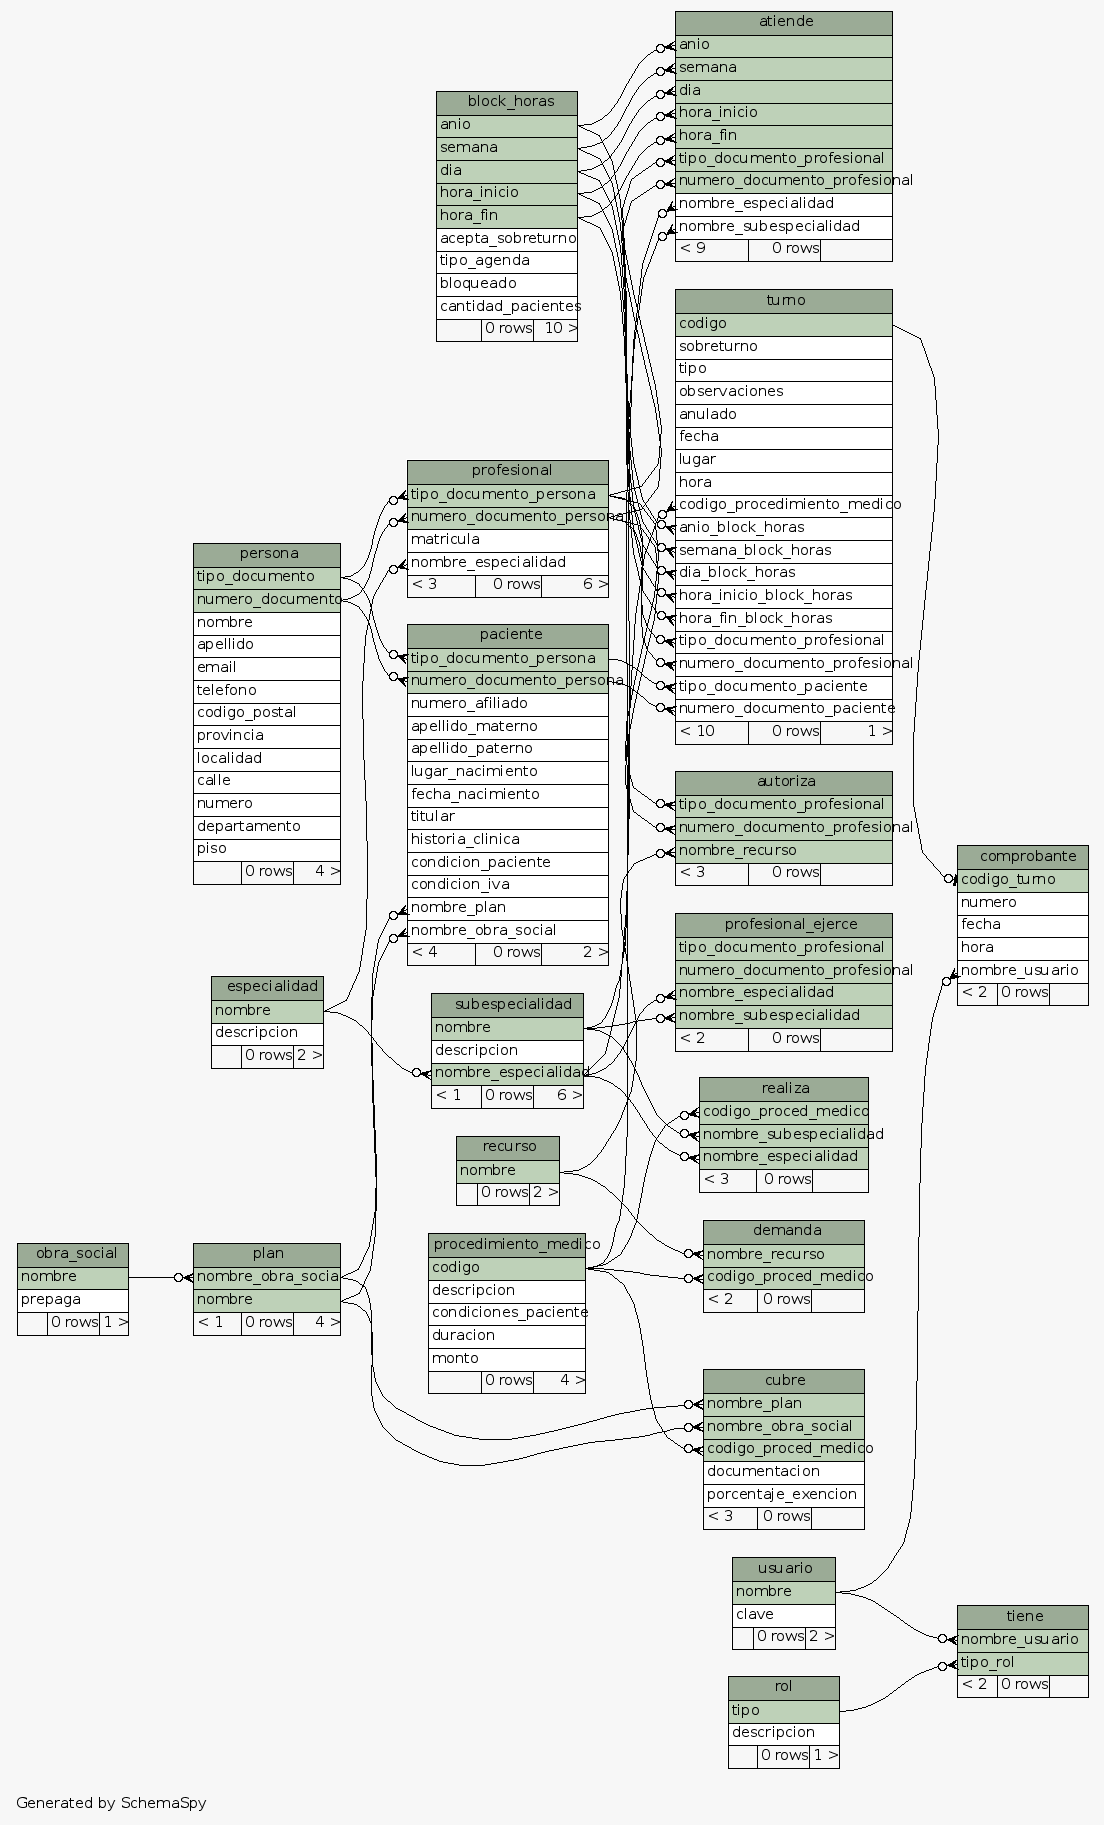
\includegraphics[width=15cm,height=25cm,angle=0]{build/images/relacional.png}
  \caption{Modelo relacional}
  \label{fig:relacional}
\end{figure}

\FloatBarrier

\subsection{\textbf{Scripts de creación}}

%A continuación se incluyen los scripts de creación de las tablas del modelo
%relacional para ser ejecutado en un sistema de bases de datos que interprete
%SQL, particularmente las instrucciones DDL de dicho lenguaje. No se incluyen
%las instrucciones, normalmente específicas al motor propiamente dicho, de
%creación de usuarios, roles, schemas y bases de datos correspondientes.

\lstinputlisting[inputencoding=latin1,language=SQL,caption={Script de definición de la base de datos}]{../scripts/script_creacion_db.sql}

\clearpage

\part{Apéndice}
\appendix

\section{Enunciado original}\label{sec:enunciado}
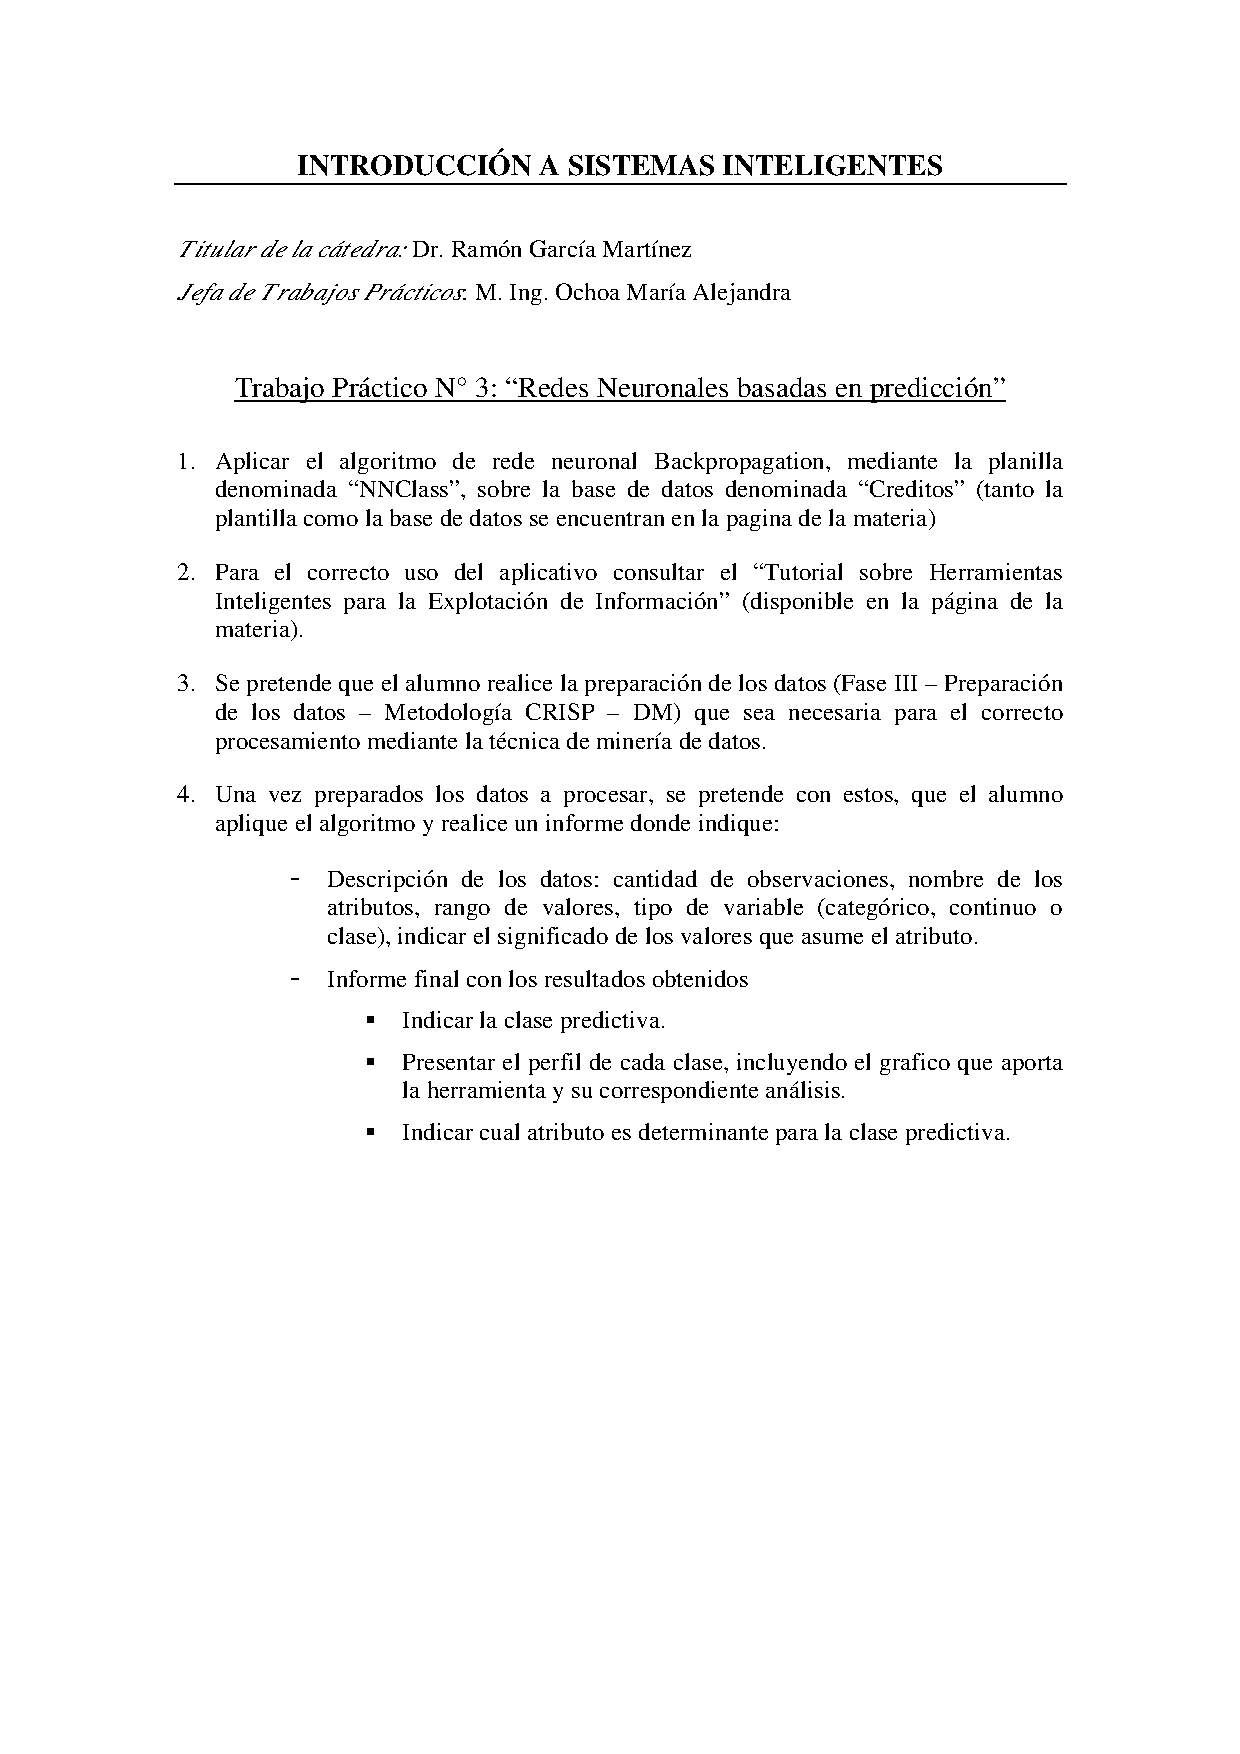
\includepdf[pages={-}, frame=true, pagecommand={}, noautoscale=true, scale=0.7]{doc/enunciado.pdf}

\clearpage

\section{\textbf{Forma de presentación del trabajo práctico}}

\begin{enumerate}
\item Presentar el diagrama de entidad - interrelación con indicaciones de restricciones 
de cardinalidad. 

\item Indicar dependencias de identidad y de existencia en el modelo. 

\item Especificar supuestos que justifiquen el modelo (Hipótesis). 

\item Presentar el diccionario de datos del diagrama con la siguiente información: 

Para cada tipo de entidad se debe especificar:

\begin{enumerate}
\item Definición. 

\item Especificación de atributos. 

\item Especificación de identificador único. 

Para cada tipo de interrelación se debe especificar: ~ 

\item Definición. 

\item Especificación de atributos. 

\item Especificación de identificador único. 
\end{enumerate}

\item Presentar el modelo Relacional ( \texttt{"}de tablas\texttt{"} )~ indicando 
para cada esquema de relación: 

\begin{enumerate}
\item Atributos 

\item Claves candidatas

\item Clave primaria

\item Claves foráneas 

\item Atributos que pueden tomar valores nulos

\item Realice el diagrama del Modelo de Tablas

\item Sentencias DDL
\end{enumerate}
\end{enumerate}

Nota: en los casos en que existan diferentes alternativas para efectuar la transformación 
de MER al modelo de tablas, elegir una única alternativa y enumerar las ventajas 
y desventajas de la alternativa elegida. \pagebreak{}\label{HToc293405800}

\end{document}
